\documentclass[10pt,twoside]{report}

% Pengaturan ukuran halaman dan margin
\usepackage[a4paper,top=25mm,left=25mm,right=20mm,bottom=25mm]{geometry}

% Pengaturan ukuran spasi
\usepackage[doublespacing]{setspace}

% Judul dokumen
\title{Buku Tutorial Virtual Mouse Using Hand Gesture Python}
\author{Musk, Elon Reeve \and Kjellberg, Felix Arvid Ulf}

% Pengaturan format bahasa
\usepackage[indonesian]{babel}

% Pengaturan detail pada file PDF
\usepackage[pdfauthor={\@author},bookmarksnumbered,pdfborder={0 0 0}]{hyperref}

% Pengaturan jenis karakter
\usepackage[utf8]{inputenc}

% Pengaturan ukuran indentasi paragraf
\setlength{\parindent}{2em}

% Pengaturan ukuran spasi paragraf
\setlength{\parskip}{0.5ex}

% Package lainnya
\usepackage{etoolbox} % Mengubah fungsi default
\usepackage{enumitem} % Pembuatan list
\usepackage{lipsum} % Pembuatan template kalimat
\usepackage{graphicx} % Input gambar
\usepackage{longtable} % Pembuatan tabel
\usepackage[table,xcdraw]{xcolor} % Pewarnaan tabel
\usepackage[numbers]{natbib} % Kutipan artikel
\usepackage{eso-pic} % Pembuatan background
\usepackage{changepage} % Pembuatan teks kolom
\usepackage{wrapfig} % Wrapping gambar

% Definisi untuk "Hati ini sengaja dikosongkan"
\def\kosong{
  \vspace*{\fill}
  \begin{center}\textit{Halaman ini sengaja dikosongkan}\end{center}
  \vfill
}
\patchcmd{\cleardoublepage}{\hbox{}}{\kosong}{}{}

% Pengaturan penomoran halaman
\usepackage{fancyhdr}
\fancyhf{}
\renewcommand{\headrulewidth}{0pt}
\pagestyle{fancy}
\fancyfoot[CE,CO]{\thepage}
\patchcmd{\chapter}{plain}{fancy}{}{}
\patchcmd{\chapter}{empty}{plain}{}{}

% Pengaturan format judul bab
\usepackage{titlesec}
\titleformat{\chapter}[display]{\bfseries\Large}{BAB \centering\Roman{chapter}}{0ex}{\vspace{0ex}\centering}[\vspace{2ex}]
\titleformat{\section}{\bfseries\large}{\MakeUppercase{\thesection}}{1ex}{}
\titleformat{\subsection}{\bfseries\large}{\MakeUppercase{\thesubsection}}{1ex}{}
\titleformat{\subsubsection}{\bfseries\large}{\MakeUppercase{\thesubsubsection}}{1ex}{}
\titlespacing{\chapter}{0ex}{0ex}{2ex}
\titlespacing{\section}{0ex}{2ex}{1ex}
\titlespacing{\subsection}{0ex}{1ex}{0.5ex}
\titlespacing{\subsubsection}{0ex}{1ex}{0.5ex}

% Pengaturan persamaan
\newenvironment{conditions}
{\par\vspace{\abovedisplayskip}\noindent
  \tabularx{\columnwidth}{>{$}l<{$} @{${}={}$} >{\raggedright\arraybackslash}X}}
{\endtabularx\par\vspace{\belowdisplayskip}}

% Pengaturan format baris program
\usepackage{listings}
\definecolor{comment}{RGB}{0,128,0}
\definecolor{string}{RGB}{255,0,0}
\definecolor{keyword}{RGB}{0,0,255}
\lstdefinestyle{codestyle}{
  commentstyle=\color{comment},
  stringstyle=\color{string},
  keywordstyle=\color{keyword},
  basicstyle=\footnotesize\ttfamily,
  numbers=left,
  numberstyle=\tiny,
  numbersep=5pt,
  frame=lines,
  breaklines=true,
  prebreak=\raisebox{0ex}[0ex][0ex]{\ensuremath{\hookleftarrow}},
  showstringspaces=false,
  upquote=true,
  tabsize=2,
}
\lstset{style=codestyle}

% Isi keseluruhan dokumen
\begin{document}

  % Nomor halaman pembuka dimulai dari sini
  \pagenumbering{roman}

  % Sampul luar
  \AddToShipoutPictureBG*{
  \AtPageLowerLeft{
    % Ubah nilai berikut jika posisi horizontal background tidak sesuai
    \hspace{-3.5mm}

    % Ubah nilai berikut jika posisi vertikal background tidak sesuai
    \raisebox{0mm}{
      
\includegraphics[width=\paperwidth,height=\paperheight]{sampul/sampul-luar.png}
    }
  }
}

% Menyembunyikan nomor halaman
\thispagestyle{empty}

% Pengaturan margin untuk menyesuaikan konten sampul
\newgeometry{top=70mm,left=25mm,right=20mm,bottom=25mm}

\begin{flushleft}

  % Pengaturan jenis dan warna teks yang digunakan
  \sffamily\color{white}
  % Ubah kalimat berikut sesuai dengan judul topik kerja praktik
  \begin{center}
    \vspace{30ex}
    \noindent{\large \textbf{VIRTUAL MOUSE USING HAND GESTURE PYTHON}}
    \vspace{30ex}
  \end{center}

  \begin{adjustwidth}{-2mm}{}
    \begin{tabular}{lcp{0.7\linewidth}}
      % Ubah kalimat-kalimat berikut sesuai dengan nama dan NRP mahasiswa pertama
      \textbf{Argya Rijal Rafi} & & \textbf{NPM 1204062} \\
      % Ubah kalimat-kalimat berikut sesuai dengan nama dan NRP mahasiswa kedua
      \textbf{Guna Darma} & & \textbf{NPM 1204062} \\
    \end{tabular}
  \end{adjustwidth}
  \vspace{4ex}

  \noindent\textbf{Dosen Pembimbing} \\
  % Ubah kalimat berikut sesuai dengan nama dosen pembimbing
  \textbf{Rolly Awangga, S.T., M.T.}
  \vspace{10ex}

  % Ubah kalimat berikut sesuai dengan nama fakultas
  \textbf{Teknik Informatika} \\
  \textbf{Politeknik Pos Indonesia} \\
  % Ubah kalimat berikut sesuai dengan tempat dan tahun pembuatan buku
  \textbf{Bandung 2021}

\end{flushleft}

\restoregeometry

  \cleardoublepage

  % Sampul dalam
  \AddToShipoutPictureBG*{
  \AtPageLowerLeft{
    % Ubah nilai berikut jika posisi horizontal background tidak sesuai
    \hspace{-3.5mm}

    % Ubah nilai berikut jika posisi vertikal background tidak sesuai
    \raisebox{0mm}{
      
\includegraphics[width=\paperwidth,height=\paperheight]{sampul/sampul-dalam.png}
    }
  }
}

% Pengaturan margin untuk menyesuaikan konten sampul
\newgeometry{top=70mm,left=25mm,right=20mm,bottom=25mm}

\begin{flushleft}

  % Pengaturan jenis teks yang digunakan
  \sffamily

  % Ubah penomoran buku berikut sesuai dengan yang ditentukan oleh departemen
  \noindent\textbf{PROJECT 2 TEKNIK INFORMATIKA}
  \vspace{4ex}

  % Ubah kalimat berikut sesuai dengan nama perusahaan tempat kerja praktik
  \noindent{\large \textbf{POLITEKNIK POS INDONESIA}} \\
  % Ubah tanggal berikut sesuai dengan waktu berlangsungnya kerja praktik
  \textbf{\today}
  \vspace{6ex}

  % Ubah kalimat berikut sesuai dengan judul topik kerja praktik
  \noindent{\large \textbf{PEMBUATAN VIRTUAL MOUSE USING HAND GESTURE PYTHON}}
  \vspace{6ex}

  \begin{adjustwidth}{-2mm}{}
    \begin{tabular}{lcp{0.7\linewidth}}
      % Ubah kalimat-kalimat berikut sesuai dengan nama dan NRP mahasiswa pertama
      \textbf{ARGYA RIJAL RAFI} & & \textbf{NPM 1204062} \\
      % Ubah kalimat-kalimat berikut sesuai dengan nama dan NRP mahasiswa kedua
      \textbf{GUNA DARMA} & & \textbf{NPM 1204071} \\
    \end{tabular}
  \end{adjustwidth}
  \vspace{4ex}

  \noindent
  \textbf{Dosen Pembimbing} \\
  % Ubah kalimat berikut sesuai dengan nama dosen pembimbing
  \textbf{ROLLY AWANGGA, S.T., M.T.}
  \vspace{10ex}

  % Ubah kalimat berikut sesuai dengan nama fakultas
  \textbf{D4 TEKNIK INFORMATIKA} \\
  \textbf{POLITEKNIK POS INDONESIA} \\
  % Ubah kalimat berikut sesuai dengan tempat dan tahun pembuatan buku
  \textbf{Bandung 2021}

\end{flushleft}

\restoregeometry

  \cleardoublepage

  % Kata pengantar
  \begin{center}
  \Large\textbf{KATA PENGANTAR}
\end{center}
\vspace{2ex}

\addcontentsline{toc}{chapter}{KATA PENGANTAR}

% Ubah paragraf-paragraf berikut sesuai dengan yang ingin diisi pada kata pengantar

Puji dan syukur kehadirat \lipsum[1][1-5]

Penelitian ini disusun dalam rangka \lipsum[2][1-5]
Oleh karena itu, penulis mengucapkan terima kasih kepada:

\begin{enumerate}[nolistsep]

  \item Keluarga, Ibu, Bapak dan Saudara tercinta yang telah \lipsum[3][1-2]

  \item Bapak Nikola Tesla, S.T., M.T., selaku \lipsum[3][3-4]

  \item \lipsum[3][5-7]

\end{enumerate}

Akhir kata, semoga \lipsum[4][1-8]

\begin{flushright}
  \begin{tabular}[b]{c}
    % Ubah kalimat berikut sesuai dengan tempat, bulan, dan tahun penulisan
    Surabaya, Februari 2021
    \\
    \\
    \\
    \\
    Penulis
  \end{tabular}
\end{flushright}

  \cleardoublepage

  % Daftar isi
  \renewcommand*\contentsname{DAFTAR ISI}
  \addcontentsline{toc}{chapter}{\contentsname}
  \tableofcontents
  \cleardoublepage

  % Daftar gambar
  \renewcommand*\listfigurename{DAFTAR GAMBAR}
  \addcontentsline{toc}{chapter}{\listfigurename}
  \listoffigures
  \cleardoublepage

  % Daftar tabel
  \renewcommand*\listtablename{DAFTAR TABEL}
  \addcontentsline{toc}{chapter}{\listtablename}
  \listoftables
  \cleardoublepage

  % Nomor halaman isi dimulai dari sini
  \pagenumbering{arabic}

  % Bab 1 pendahuluan
  \chapter{VIRTUAL MOUSE USING HAND GESTURE PYTHON}

Mouse adalah salah satu penemuan yang luar biasa pada dunia tekhnologi Human-computer Interaction (HCI), saat ini mouse nirkabel atau mouse bluetooth masih menggunakan perangkat keras karena membutuhkan batrai dan kabel 	untuk menghubungkan nya ke pc. Dalam sistem virtual mouse yang diusulkan, keterbatasan ini dapat diatasi dengan menggunakan webcam atau kamera built-in untuk menangkap gerakan tangan dan mendeteksi ujung jari menggunakan visi komputer, algoritma yang digunakan dalam sistem ini menggunakan algoritma mechine learning berdasarkan gerakan tangan yang telah terdeteksi, komputer dapat dikontrol secara virtual dan dapat melakukan fungsi klik kanan, klik kiri, drag and drop, scrolling dan fungsi mouse lainya tanpa membutuhkan perangkat keras.


\section{Virtual Mouse Hand Gesture}

\begin{enumerate}
  \item \textbf{Artificial Intelegence} \\
    Artificial Intelegence (AI) adalah cabang ilmu komputer yang mensimulasikan kecerdasan yang dimiliki oleh manusia yang diimplementasikan kedalam suatu program komputer, kecerdasan buatan adalah aktivitas mesin yang menampilkan prilaku yang dianggap hampir menyerupai kecerdasan yang dimiliki oleh manusia, sehingga bisa dikatakan AI merupakan sistem atau program kompute yang mampu melakukan pekerjaan dan memutuskan sesuatu seperti layaknya manusia.
    AI juga merupakan tekhnologi yang memungkinkan mesin bisa mengerti apa yang pengguna inginkan dan butuhkan, misalnya untuk menciptakan mesin yang dapat menidentifikas suara dan mampu memberikan \textit{return} atau timbal balik dari mesin tersebut. 
  \item \textbf{Machine Learning}  \\
    Istiah \textit{mechine learning}  pertama kali dikemukakan oleh beberapa ilmuan matematika seperti Adren Marie Lagandrie, Thomas Bayes dan Andrey Mrkov pada tahun 1920-an dengan mengemukakan dasar-dasar \textit{mechine learning} dan konsepnya. sejak saat itu ML banyak yang mengembangkan. salah satu contoh dari penerapan ML yang cukup terkenal adalah \textit{deep blue} yang dibuat oleh IBM pada tahun 1996.
    Teknologi \textit{mechine learning}  adalah mesin yang dikembangkan untuk bisa belajar dengan sendirinya tanpa arahan dari pengguna atau \textit{user}, pembeljaran \textit{mechine learning}  dikembangkan berdasarkan disiplin ilmu lainya seperti statistika, matematika dan data mining sehingga mesin dapat belajar dengan menganalisis data tanpa perlu di program ulang atau diperintah.
    untuk bisa mengoprasikan \textit{mechine learning} secara optimal terdapat 3 metode yaitu: 
    \begin{figure} [ht] \centering
      % Nama dari file gambar yang diinputkan
      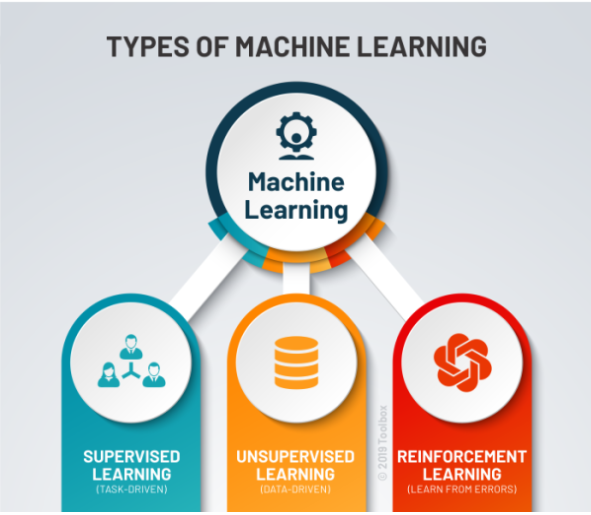
\includegraphics[scale=0.9]{gambar/metode_ML.png}
      % Keterangan gambar yang diinputkan
      \caption{tiga metode atau tipe mechine learning (Sumber: ekrut.com)}
      % Label referensi dari gambar yang diinputkan
      \label{fig:MechineLearning}
    \end{figure}
    \begin{enumerate}[nolistsep]
      \item \textit{\textbf{Supervised Learning}}\\
        Metode supervised learning dilakukan dengan pemberian label pada dataset  yang digunakan oleh machine learning dan diklasifikasikan oleh pengembang dengan memungkinkan algoritma melihat tingkat akurasi kinerjanya. Pengawasan machine learning dalam metode ini dilakukan oleh data berlabel yang nantinya membuat machine learning mempelajari apa hubungan dan ketergantungan antar data.
        Cara kerja metode ini adalah memasukkan informasi sebagai input dan data berlabel sebagai hasil atau output. Input dalam machine learning pinjaman bank misalnya dapat berupa data rinci seperti usia, gaji, jumlah pinjaman, jumlah terutan, riwayat pinjaman, dan lain sebagainya. Sedangkan output-nya dapat berupa hasil dari keseluruhan jumlah orang yang membayar pinjaman dan berapa jumlah orang gagal membayar.
      \item \textit{\textbf{Semi-supervised Learning (Unsupervised)}} \\
        Metode \textit{semi-supervised learning} bisa disebut juga sebagai metode \textit{machine learning} tanpa pengawasan. Sehingga, prosesnya dilakukan pada dataset mentah yang tidak berlabel dan algoritma \textit{machine learning} akan mencoba mengidentifikasi pola dan relasi antar data tanpa bantuan dari pengembang.
        Metode \textit{unsupervised learning} pada umumnya memang tidak ada bantuan dari manusia agar komputer benar-benar mempelajari sebuah data dan relasinya secara mandiri. Dalam kasusnya, dataset tidak berlabel dan mesin secara komputasi akan mengidentifikasi pola dalam data. \textit{Unsupervised learning} digunakan untuk memudahkan pengembang mengambil keputusan.
        Dalam kasus \textit{mechine learning} pinjaman bank tadi, sebuah \textit{unsupervised learning} dapat mendeteksi anomali atau mengungkap transaksi atau pembayaran yang curang. \textit{Unsupervised learning}  dapat secara otomatis mencari informasi setelah mengelompokkan pola dari semua data peminjam dari sebuah bank dan memunculkannya sebagai sebuah output tanpa harus memasukkan data berlabel secara rinci.
      \item \textit{\textbf{Reinforcement Learning}} \\
        Metode \textit{machine learning} yang satu ini dijalankan dengan menggunakan dataset bersistem “rewards/punishment” dan menawarkan umpan balik ke algoritma untuk belajar dari pengalamannya secara coba-coba (random). Metode “coba-coba” ini hampir sama dengan sistem pemahaman pola yang dilakukan manusia yaitu belajar dari percobaan.

        Hal ini yang lantas membuat metode ini disebut sebagai \textit{machine learning} dengan tipe penguatan pembelajaran. Algoritma dalam metode ini akan belajar secara terus-menerus dari lingkungan atau kebiasaan interaksi yang berhubungannya dengannya. Dari sana nantinya algoritma akan mendapat “rewards” atau “punishment” sebagai impresi positif dan negatif berdasarkan tindakan percobaannya.
      
        Dalam kasus machine learning pinjaman bank, algoritma reinforcement learning akan mengklasifikasikan pelanggan berisiko tinggi secara default dan akan mengelompokkan pelanggan yang gagal bayar sebagai aspek negatif secara otomatis.  
    \end{enumerate}
  \item \textbf{Deep Learning} \\ 
    Deep learning adalah salah satu subbidang dari \textit{mechine learning} yang algoritmanya terinpirasi dari otak manusia. Saat ini teknik \textit{deep learning} telah diterapkan diberbagai bidang teknologi seperti \textit{self-driving car}, \textit{deep learning} yang disusun berdasarkan arsitektur otak manusia dinamakan \textit{Artificial Neural Network} atau ANN. ia mampu belajar dan beradaptasi teradap sejumlh besar data serta menyelesaikan berbagai permasalahan yang sulit diselesaikan dengan algortma \textit{mechine learning} lainnya. 
    \begin{enumerate}[nolistsep]
      \item \textbf{\textit{Convolutional Neural Network (CNN)}}\\
        CNN terdiri dari banyak layer untuk memproses dan mengekstrak fitur dari data. Ia biasanya digunakan untuk memproses gambar dan mendeteksi objek. Saat ini, CNN banyak digunakan untuk mengidentifikasi citra satelit, citra medis, dan mendeteksi anomali.
      \item \textbf{\textit{Recurrent Neural Network (RNN)}}\\
        \textit{Recurrent Neural Networks (RNN)} merupakan salah satu bentuk arsitektur \textit{Artificial Neural Networks (ANN)} yang dirancang khusus untuk memproses data yang bersambung/ berurutan (sequential data). RNN biasanya digunakan untuk menyelesaikan permasalahan data historis atau time series, contohnya data ramalan cuaca. Selain itu, RNN juga dapat diimplementasikan pada bidang natural language understanding (pemahaman bahasa alami), misalnya  translasi bahasa.
      \item \textbf{\textit{{Long Short Term Memory Network (LTSM)}}}\\
        LSTM merupakan tipe \textit{Recurrent Neural Network} yang dapat mempelajari data historis atau time series. Ia merupakan algoritma \textit{deep learning} yang kompleks dan dapat mempelajari informasi jangka panjang dengan sangat baik. LSTM sangat powerful untuk menyelesaikan berbagai permasalahan kompleks seperti speech recognition, speech to text application, komposisi musik, dan pengembangan di bidang farmasi.
      \item \textbf{\textit{Self Organizing Maps (SOM)}}\\
        Jenis terakhir adalah \textit{self organizing maps} atau SOM. Algoritma ini mampu membuat visualisasi data secara mandiri. SOM diciptakan untuk membantu penggunanya dalam memahami data dan informasi berdimensi tinggi
    \end{enumerate}
  \item \textbf{\textit{Neural Network}}\\
    \textbf{\textit{Neural Network}} adalah kategori ilmu Soft Computing. Neural Network sebenarnya mengadopsi dari kemampuan otak manusia yang   mampu memberikan stimulasi/rangsangan, melakukan proses, dan memberikan output. Output diperoleh dari variasi stimulasi dan proses yang terjadi di dalam otak manusia. Kemampuan manusia dalam memproses informasi merupakan hasil kompleksitas proses di dalam otak. Misalnya, yang terjadi pada anak-anak, mereka mampu belajar untuk melakukan pengenalan meskipun mereka tidak mengetahui algoritma apa yang digunakan. Kekuatan komputasi yang luar biasa dari otak manusia ini merupakan sebuah keunggulan di dalam kajian ilmu pengetahuan.
    Neural Network berguna untuk:
    \begin{enumerate}[nolistsep]
      \item pengklasifikasian pola
      \item memetakan pola yang didapat dari input kedalam pola baru pada output 
      \item penyimpan pola yang akan di panggil kemabali ketika dibutuhkan
      \item memetaka pola-pola yang sejenis
      \item pengoptimas permasalahan
      \item prediksi
    \end{enumerate}
    dalam perancangan \textit{Neural Network} memiliki beberapa konsep yang mendasari terbentuknya sistem saraf buatan yang memungkinkan untuk bisa bekerja selayaknya sitem saraf otak pada manusia, Ide dasar \textit{Neural Network} dimulai dari otak manusia, dimana otak memuat  sekitar $10^{11}$ neuron. Neuron ini berfungsi memproses setiap informasi yang masuk. Satu neuron memiliki 1 akson, dan minimal 1 dendrit. Setiap sel syaraf terhubung dengan syaraf lain, jumlahnya mencapai sekitar $10^{4}$ sinapsis. Masing-masing sel itu saling berinteraksi satu sama lain yang menghasilkan kemampuan tertentu pada kerja otak manusia. 
    proses yang terjadi pada otak dimana sebuah neuron menerima impuls dari neuron lain melalui dendrit dan mengirimkan sinyal yang dihasilkan oleh badan sel melalui akson. Akson dari sel syaraf ini bercabang-cabang dan berhubungan dengan dendrit dari sel syaraf lain dengan cara mengirimkan impuls melalui sinapsis. Sinapsis adalah unit fungsional antara 2 buah sel syaraf, misal A dan B, dimana yang satu adalah serabut akson dari neuron A dan satunya lagi adalah dendrit dari neuron B. Kekuatan sinapsis bisa menurun/meningkat tergantung seberapa besar tingkat propagasi (penyiaran) sinyal yang diterimanya. Impuls-impuls sinyal (informasi) akan diterima oleh neuron lain jika memenuhi batasan tertentu, yang sering disebut dengan nilai ambang (threshold).
    \begin{figure} [ht] \centering
      % Nama dari file gambar yang diinputkan
      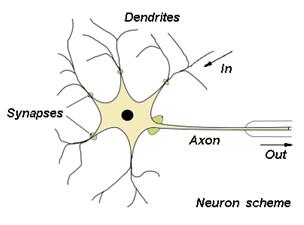
\includegraphics[scale=0.9]{gambar/neuron.jpg}
      % Keterangan gambar yang diinputkan
      \caption{Sistem Neuron Pada Otak manusia (Sumber: socs.binus.ac.id)}
      % Label referensi dari gambar yang diinputkan
      \label{fig:MechineLearning}
    \end{figure}\\
    mengikut pada gambar diatas, ada beberapa bagian otak manusia:
    \begin{enumerate}[nolistsep]
      \item Dendrit (Dendrites) berfungsi untuk mengirimkan impuls yang diterima ke badan sel syaraf.
      \item Akson (Axon) berfungsi untuk mengirimkan impuls dari badan sel ke jaringan lain
      \item Sinapsis berfungsi sebagai unit fungsional di antara dua sel syaraf.
    \end{enumerate}
\end{enumerate}



  % Bab 2 profil perusahaan
  \chapter{PENGENALAN BAHASA PEMOGRAMAN}

% Ubah konten-konten berikut sesuai dengan yang ingin diisi pada bab ini

\section{Sejarah PT. NASA}

PT. NASA berdiri pada \lipsum[11]

\lipsum[12][1-10]

\section{Visi dan Misi}

PT. NASA memiliki \lipsum[13][1-3] sebagai berikut:

\begin{enumerate}[nolistsep]

  \item \textbf{Visi PT. NASA}

  Menjadi \lipsum[13][4-7]

  \item \textbf{Misi PT. NASA}

  \begin{enumerate}[nolistsep]

    \item Membuat \lipsum[13][8-9]

    \item \lipsum[13][10-12]

  \end{enumerate}

\end{enumerate}

\section{Struktur Organisasi}

Struktur Organisasi dari \lipsum[14][1-8]

% Contoh input gambar dengan format *.png
\begin{figure} [ht] \centering
  % Nama dari file gambar yang diinputkan
  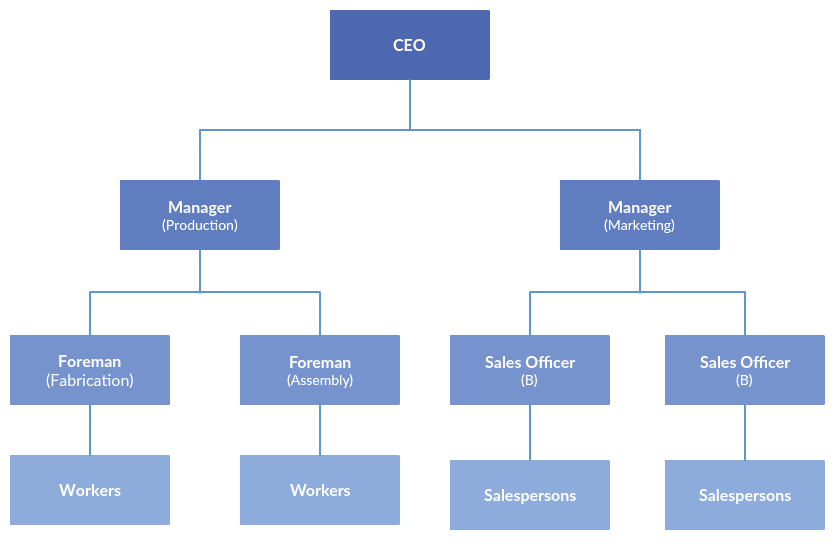
\includegraphics[scale=0.4]{gambar/organization-structure.png}
  % Keterangan gambar yang diinputkan
  \caption{Struktur organisasi PT. NASA}
  % Label referensi dari gambar yang diinputkan
  \label{fig:OrganizationStructure}
\end{figure}

% Contoh penggunaan referensi dari gambar yang diinputkan
Seperti yang bisa dilihat pada Gambar \ref{fig:OrganizationStructure}, \lipsum[15]

  \cleardoublepage

  % Bab 3 tunjauan pustaka
  % Ubah kalimat sesuai dengan judul dari bab ini
\chapter{TINJAUAN PUSTAKA}

% Ubah konten-konten berikut sesuai dengan yang ingin diisi pada bab ini

\section{Roket Luar Angkasa}

% Contoh input gambar dengan format *.jpg
\begin{figure} [ht] \centering
  % Nama dari file gambar yang diinputkan
  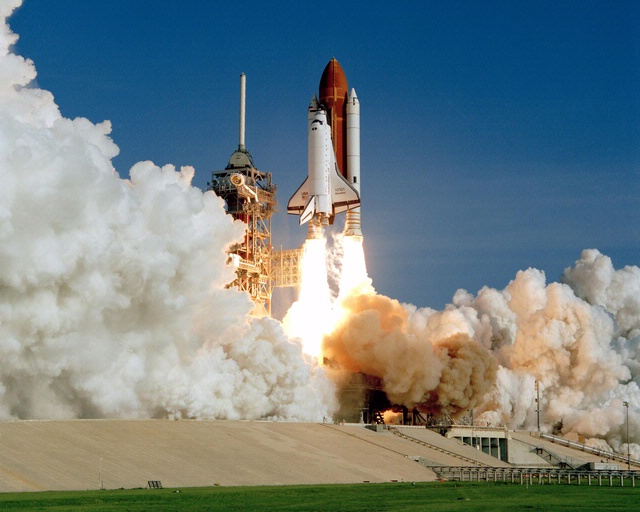
\includegraphics[scale=0.3]{gambar/space-shuttle.jpg}
  % Keterangan gambar yang diinputkan
  \caption{Peluncuran pesawat luar angkasa Discovery \citep{DiscoverySpaceShuttle}}
  % Label referensi dari gambar yang diinputkan
  \label{fig:SpaceShuttle}
\end{figure}

Roket luar angkasa merupakan \lipsum[16][1-10]

% Contoh penggunaan referensi dari gambar yang diinputkan
\emph{Discovery}, Gambar \ref{fig:SpaceShuttle}, merupakan \lipsum[17][1-9]

\section{Gravitasi}

Gravitasi merupakan \lipsum[18][1-10]

\subsection{Hukum Newton}

% Contoh penggunaan referensi dari pustaka
Newton \citep{Newton1687} pernah merumuskan bahwa \lipsum[19]
% Contoh penggunaan referensi dari persamaan
Kemudian menjadi persamaan seperti pada persamaan \ref{eq:FirstNewtonLaw}.

% Contoh pembuatan persamaan
\begin{equation}
  % Label referensi dari persamaan yang dibuat
  \label{eq:FirstNewtonLaw}
  % Baris kode persamaan yang dibuat
  \sum \mathbf{F} = 0\; \Leftrightarrow\; \frac{\mathrm{d} \mathbf{v} }{\mathrm{d}t} = 0.
\end{equation}

\subsection{Anti Gravitasi}

Anti gravitasi merupakan \lipsum[20]

  \cleardoublepage

  % Bab 4 desain dan implementasi
  % Ubah kalimat sesuai dengan judul dari bab ini
\chapter{DESAIN DAN IMPLEMENTASI}

% Ubah konten-konten berikut sesuai dengan yang ingin diisi pada bab ini

\section{Deskripsi Sistem}

Sistem akan dibuat dengan \lipsum[21][1-12]

\section{Implementasi Alat}

Alat diimplementasikan dengan \lipsum[22]

% Contoh pembuatan code snippet
\begin{lstlisting}[
  language=C++,
  label={lst:Hello World},
  caption={Program hello world}
]
#include <iostream>

int main() {
    std::cout << "Hello World!";
    return 0;
}
\end{lstlisting}

% Contoh penggunaan referensi dari code snippet yang diinputkan
Seperti contoh pada baris program Listing \ref{lst:Hello World} dan Listing \ref{lst:PrimeNumber}, \lipsum[23]

% Contoh input code snippet
\lstinputlisting[
  % Bahasa yang digunakan oleh code snippet
  language=Python,
  % Label referensi dari code snippet yang diinputkan
  label={lst:PrimeNumber},
  % Keterangan dari code snippet yang diinputkan
  caption={Program perhitungan bilangan prima}
% Nama dari file code snippet yang diinputkan
]{program/prime-number.py}

  \cleardoublepage

  % Bab 5 pengujian dan evaluasi
  % Ubah kalimat sesuai dengan judul dari bab ini
\chapter{PENGUJIAN DAN EVALUASI}

% Ubah konten-konten berikut sesuai dengan yang ingin diisi pada bab ini

\section{Skenario Pengujian}

Pengujian dilakukan dengan \lipsum[24]

\section{Evaluasi Pengujian}

Dari pengujian yang \lipsum[25][1-10]

% Contoh input konten dari file terpisah
%Contoh pembuatan tabel
\begin{longtable}{|l|l|l|}
  % Keterangan dari tabel yang dibuat
  \caption{Hasil Pengukuran Energi dan Kecepatan}
  % Label referensi dari tabel yang dibuat
  \label{tb:EnergiKecepatan}\\
  % Isi dari tabel yang dibuat
  \hline
  \rowcolor[HTML]{C0C0C0}
  \textbf{Energi} & \textbf{Jarak Tempuh} & \textbf{Kecepatan} \\ \hline
  10 J & 1000 M & 200 M/s \\ \hline
  20 J & 2000 M & 400 M/s \\ \hline
  30 J & 4000 M & 800 M/s \\ \hline
  40 J & 8000 M & 1600 M/s \\ \hline
\end{longtable}


% Contoh penggunaan referensi dari tabel yang dibuat
Sesuai dengan hasil pada Tabel \ref{tb:EnergiKecepatan}, didapatkan bahwa energi yang \lipsum[26]

  \cleardoublepage

  % Bab 6 kesimpulan dan saran
  % Ubah kalimat sesuai dengan judul dari bab ini
\chapter{KESIMPULAN DAN SARAN}

% Ubah konten-konten berikut sesuai dengan yang ingin diisi pada bab ini

\section{Kesimpulan}

Kesimpulan yang kami peroleh dari \lipsum[28][1-3] adalah:

\begin{enumerate}[nolistsep]

  \item Pembuatan \lipsum[29][1-3]

  \item \lipsum[29][4-6]

  \item \lipsum[29][7-9]

\end{enumerate}

\section{Saran}

Saran yang kami ajukan dalam \lipsum[30][1-2] antara lain:

\begin{enumerate}[nolistsep]

  \item Sebaiknya \lipsum[31][1-3]

  \item \lipsum[31][4-6]

  \item \lipsum[31][7-9]

\end{enumerate}

  \cleardoublepage

  % Daftar pustaka
  \renewcommand\bibname{DAFTAR PUSTAKA}
  \addcontentsline{toc}{chapter}{\bibname}
  \bibliographystyle{unsrtnat}
  \bibliography{pustaka/pustaka.bib}
  \cleardoublepage

  % Biografi penulis
  \begin{center}
  \Large\textbf{BIOGRAFI PENULIS}
\end{center}
\vspace{2ex}

\addcontentsline{toc}{chapter}{BIOGRAFI PENULIS}

\begin{wrapfigure}{L}{0.3\textwidth}
  \centering
  \vspace{-3ex}
  %  nama file gambar berikut adalah nama file foto dari mahasiswa pertama
  
\includegraphics[width=0.3\textwidth]{gambar/elon.jpg}
  \vspace{-4ex}
\end{wrapfigure}

% kalimat berikut adalah biografi dari mahasiswa pertama
\noindent Argya Rijal Rafi, lahir pada \lipsum[1]

\vspace{2ex}

\begin{wrapfigure}{L}{0.3\textwidth}
  \centering
  \vspace{-3ex}
  % nama file gambar berikut adalah nama file foto dari mahasiswa kedua
  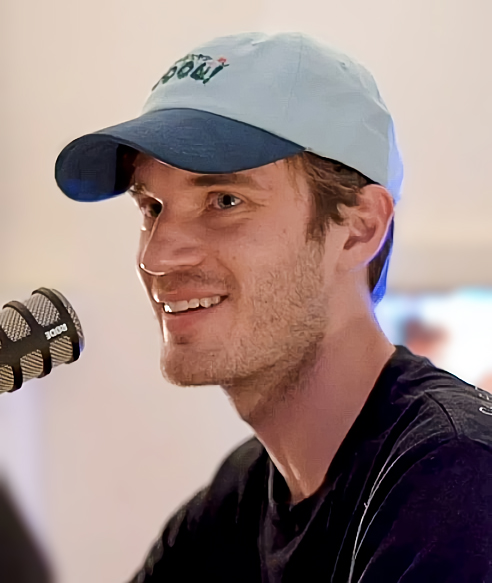
\includegraphics[width=0.3\textwidth]{gambar/felix.jpg}
  \vspace{-4ex}
\end{wrapfigure}

% kalimat berikut adalah biografi dari mahasiswa kedua
\noindent Guna Darma, lahir pada \lipsum[2]

  \cleardoublepage

\end{document}
